\subsection{UART}
\begin{frame}
  \frametitle{UART(УАПП универсальный асинхронный приемопередатчик)}
  \begin{columns}
    \column{4cm}
    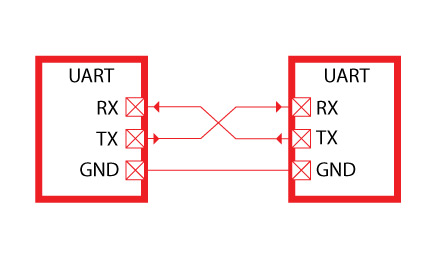
\includegraphics[width=4cm]{./slides/hardware_protocols/uart_bus.jpg}
    \column{4.5cm}
    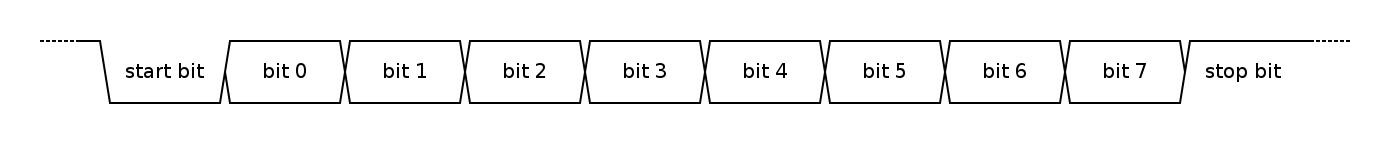
\includegraphics[width=5cm]{./slides/hardware_protocols/UART_timing_diagram.png}
  \end{columns}
\end{frame}

\begin{frame}
  \frametitle{UART:свойства}
  \begin{columns}
    \column{4cm}
    \begin{center}
      {\bf\large Достоинства}
    \end{center}
    \begin{itemize}
       \item Отн. быстрый
       \item Мало проводов
    \end{itemize}
    \column{4cm}
    \begin{center}
      {\bf\large Недостатки}
    \end{center}
    \begin{itemize}
       \item Боится погрешности часов 
       \item Асинхронность менее надежна
       \item Peer2peer
    \end{itemize}
  \end{columns}
  \begin{center}
    {\bf\large Типичное применение}
  \end{center}
  Интерфейс отладки (консоль), GPS, модемы
\end{frame}

\subsection{SPI}
\begin{frame}
  \frametitle{SPI}
  \begin{columns}
    \column{4cm}
    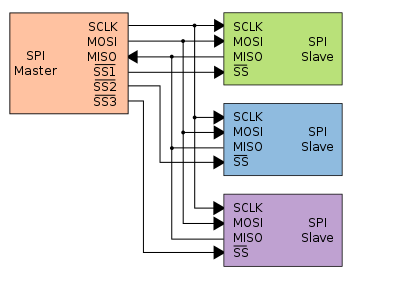
\includegraphics[width=4cm]{./slides/hardware_protocols/SPI_three_slaves.png}
    \column{4cm}
    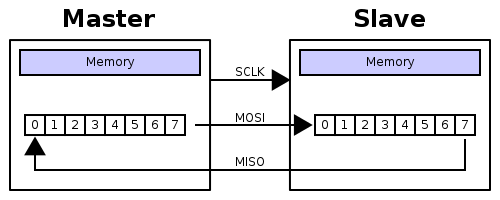
\includegraphics[width=4cm]{./slides/hardware_protocols/SPI_8-bit_circular_transfer.png}
  \end{columns}
  \begin{center}
    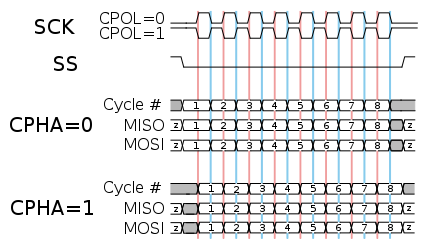
\includegraphics[height=3cm]{./slides/hardware_protocols/SPI_timing_diagram2.png}
  \end{center}
\end{frame}

\begin{frame}
  \frametitle{Логический анализатор: SPI CPOL=0 CPHA=1}
  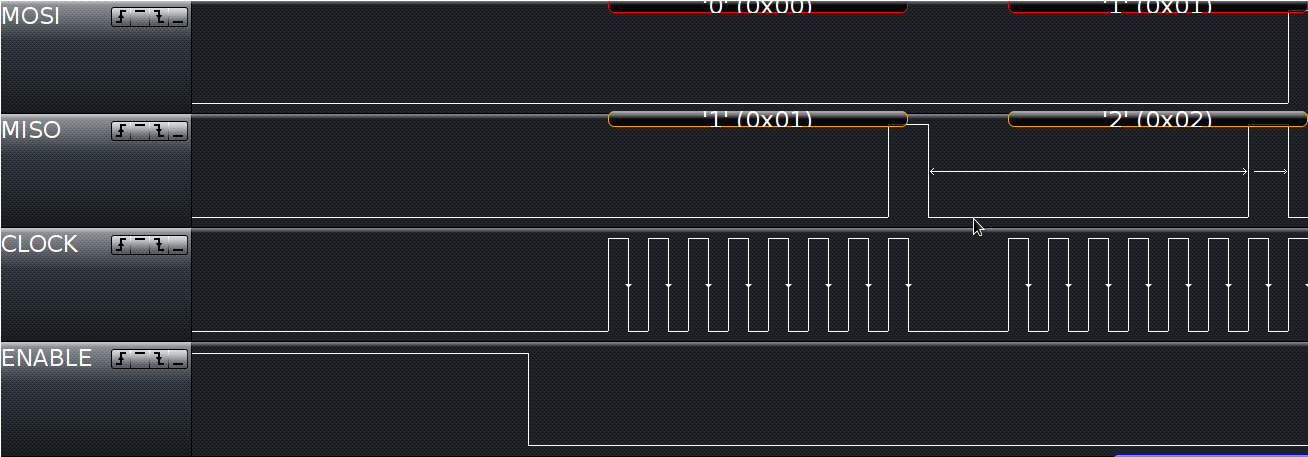
\includegraphics[width=12cm]{./slides/hardware_protocols/spi_proto_cpol0_cpha1.png}
\end{frame}

\begin{frame}
  \frametitle{Логический анализатор: SPI CPOL=0 CPHA=0}
  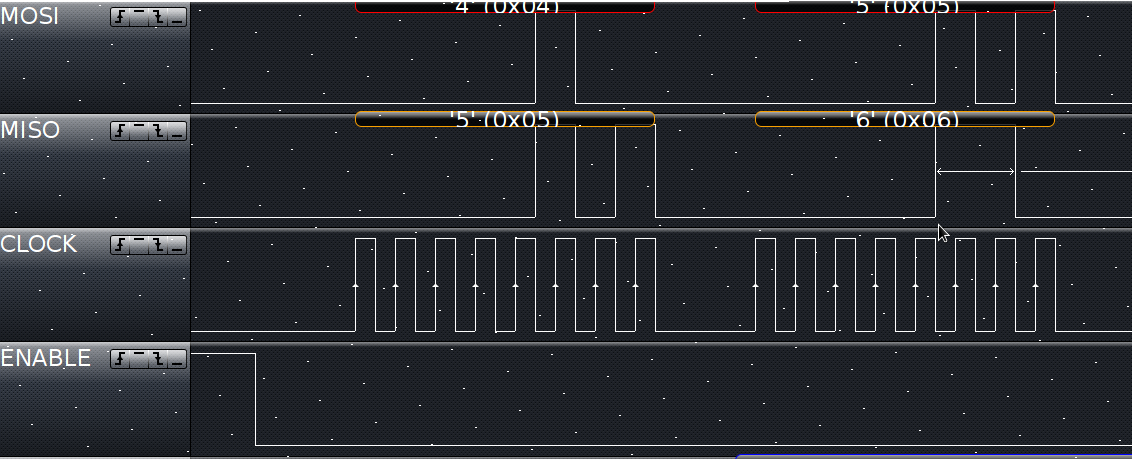
\includegraphics[width=12cm]{./slides/hardware_protocols/spi_proto_cpol0_cpha0.png}
\end{frame}

\begin{frame}
  \frametitle{Логический анализатор: SPI CPOL=1 CPHA=0}
  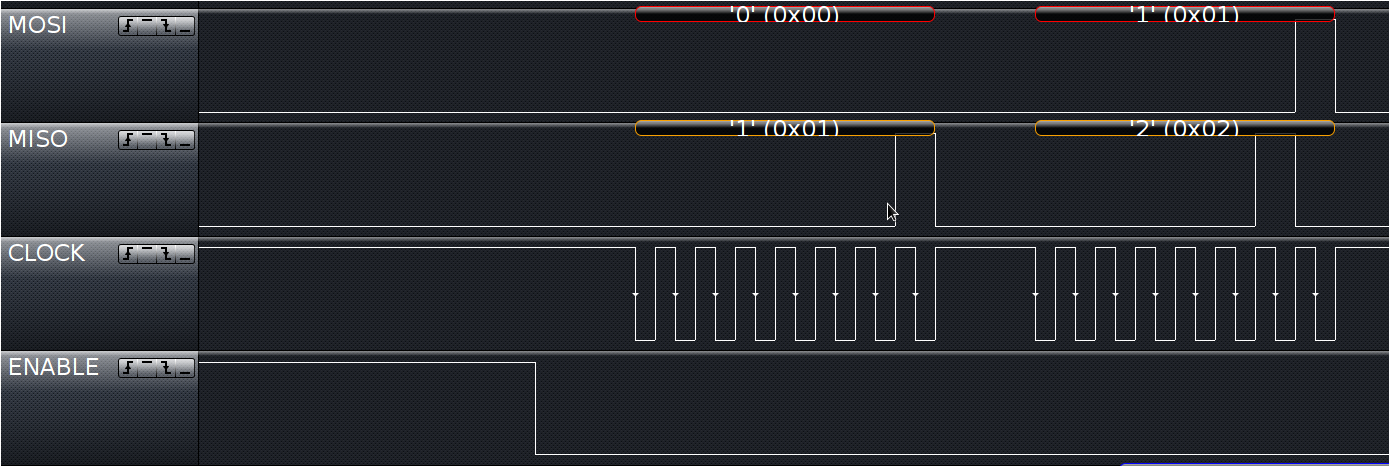
\includegraphics[width=12cm]{./slides/hardware_protocols/spi_proto_cpol1_cpha0.png}
\end{frame}


\begin{frame}
  \frametitle{SPI:свойства}
  \begin{columns}
    \column{4cm}
    \begin{center}
      {\bf\large Достоинства}
    \end{center}
    \begin{itemize}
       \item Быстрый
       \item Синхронный
       \item Простой
    \end{itemize}
    \column{4cm}
    \begin{center}
      {\bf\large Недостатки}
    \end{center}
    \begin{itemize}
       \item Много проводов (SS)
    \end{itemize}
  \end{columns}
  \begin{center}
    {\bf\large Типичное применение}
  \end{center}
  Взаимодействие с датчиками, взаимодействие с flash памятью, взаимодействие с некоторыми ethernet контроллерами
\end{frame}

\subsection{I$^2$C}   
\begin{frame}
  \frametitle{I$^2$C}
  \begin{center}
    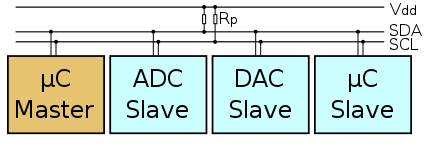
\includegraphics[height=3cm]{./slides/hardware_protocols/I2C.png}
    \vspace{0.3cm}

    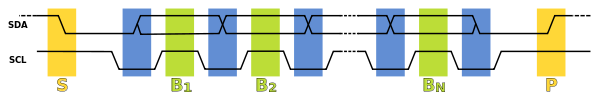
\includegraphics[height=1.5cm]{./slides/hardware_protocols/600px-I2C_data_transfer.png}
  \end{center}
\end{frame}

\begin{frame}
  \frametitle{I$^2$C: Логический анализатор: чтение}
  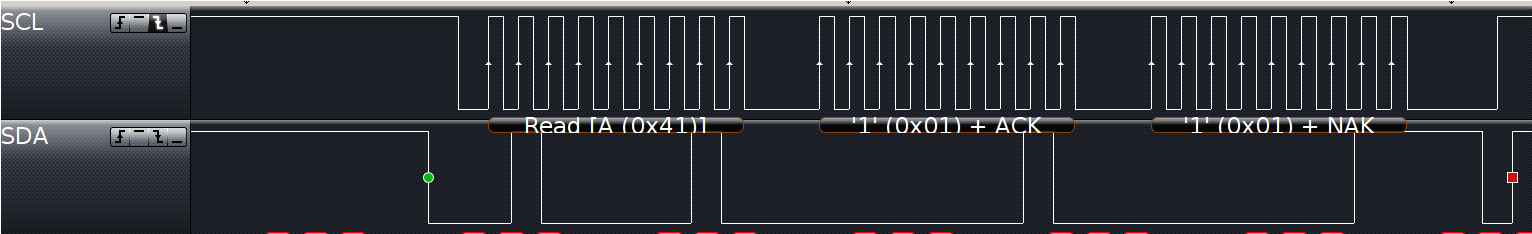
\includegraphics[width=12cm]{./slides/hardware_protocols/i2c_read.png}
\end{frame}

\begin{frame}
  \frametitle{I$^2$C:свойства}
  \begin{columns}
    \column{4cm}
    \begin{center}
      {\bf\large Достоинства}
    \end{center}
    \begin{itemize}
       \item Много периферии на три провода
       \item Синхронный
    \end{itemize}
    \column{4cm}
    \begin{center}
      {\bf\large Недостатки}
    \end{center}
    \begin{itemize}
       \item Отн. медленный
       \item Сложный
    \end{itemize}
  \end{columns}
  \begin{center}
    {\bf\large Типичное применение}
  \end{center}
  Взаимодействие с датчиками: гироскоп, термометр, АЦП, магнетометр; часть протокола HDMI
\end{frame}

\subsection{GPIO}
\begin{frame}
  \frametitle{GPIO}
  \textbf{GPIO(Интерфейс ввода/вывода общего назначения)} -- универсальный интерфейс, в котором установка выводов процессора в логические состояния полностью контролируется программно.
  

  \begin{columns}
    \column{4cm}
    \begin{center}
      {\bf\large Достоинства}
    \end{center}
    \begin{itemize}
       \item Наиболее универсальный
    \end{itemize}
    \column{4cm}
    \begin{center}
      {\bf\large Недостатки}
    \end{center}
    \begin{itemize}
       \item Тратятся дорогие циклы процессора
    \end{itemize}
  \end{columns}
  \begin{center}
    {\bf\large Типичное применение}
  \end{center}
  Индикаторы, включатели/выключатели, прием данных от кнопок, реализация отсутствующих железных интерфейсов

\end{frame}
\subsection{USB}
\begin{frame}
  \frametitle{USB}
  \begin{columns}
    \column{4cm}
    \begin{center}
      {\bf\large Достоинства}
    \end{center}
    \begin{itemize}
       \item Универсальный
       \item Быстрый
    \end{itemize}
    \column{4cm}
    \begin{center}
      {\bf\large Недостатки}
    \end{center}
    \begin{itemize}
       \item Дорогие контроллеры
       \item Очень сложный
    \end{itemize}
  \end{columns}
  \begin{center}
    {\bf\large Типичное применение}
  \end{center}
  Взаимодействие с пользователем (USB HID), взаимодействие с flash хранилищами (USB Storage), передача медиаданных (USB UVC, звуковые карты), 
\end{frame}
